\documentclass[zihao=-4,a4paper,fontset=none]{ctexart}

\usepackage{hyperref}
\usepackage[dvipsnames,svgnames,x11names,table]{xcolor}
\usepackage{calc}
\usepackage{graphicx}
\usepackage{tikz}
\usetikzlibrary{backgrounds,calc,shadows,positioning,fit}
\usepackage{fontspec}
\usepackage{fontawesome5}
\usepackage[explicit]{titlesec}
\usepackage{enumitem}
\newcommand*\circled[1]{\tikz[baseline=(char.base)]{
            \node[shape=circle,draw,inner sep=1pt] (char) {#1};}}
%  https://tex.stackexchange.com/questions/7032/good-way-to-make-textcircled-numbers

\newcommand*{\eitemi}{\tikz \draw [baseline, ball color=main,draw=none] circle (3pt);}
\newcommand*{\eitemii}{\tikz \draw [baseline, fill=main,draw=none,circular drop shadow] circle (3pt);}
\newcommand*{\eitemiii}{\tikz \draw [baseline, fill=main,draw=none] circle (3pt);}
\setlist[enumerate,1]{label=\color{main}\arabic*.}
\setlist[enumerate,2]{label=\color{main}(\alph*).}
\setlist[enumerate,3]{label=\color{main}\Roman*.}
\setlist[enumerate,4]{label=\color{main}\Alph*.}
\setlist[itemize,1]{label={\eitemi}}
\setlist[itemize,2]{label={\eitemii}}
\setlist[itemize,3]{label={\eitemiii}}
\setlist[itemize]{nosep,                     % 取消 itemize 的默认间距
    before={\vspace*{-\parskip}},          % 取消 itemize 和后续段落之间的空白
    leftmargin=*}		                    % 取消 itemize 的左边距
\setlist[enumerate]{leftmargin=*}	        % 取消 enumerate 的左边距
\usepackage{fancybox}
\usepackage{newtxmath}
\usepackage{tcolorbox}
\hypersetup{hidelinks}
\pagecolor{lightgray!10}
%%%%%%%%%%%%%%%%%%%%
% 设置
%%%%%%%%%%%%%%%%%%%%

\setlength{\parindent}{0pt}					% 取消全局段落缩进
\pagenumbering{gobble}						% 取消页码显示
\renewcommand{\arraystretch}{1.2}           % 设置表格行间距
\linespread{1.25}                           % 设置正文行间距

\titleformat{\section}					    % 将原标题前面的数字取消了
  {\LARGE\bfseries\raggedright} 		      % 字体改为 LARGE,bold,左对齐
  {}{0em}                      			  % 可用于添加全局标题前缀
  {\protect\tcbox[size=small,boxrule=0mm,arc=3pt,colback=main!10,nobeforeafter]{#1}}                           			  % 可用于添加代码
  [\vspace{-0.1em}{\color{main}\titlerule}]     % 标题下方加一条线
\titlespacing*{\section}{0cm}{*1.2}{*1.2}	% 标题左边留白,上方,下方

\usepackage[
	a4paper,
	left=1.2cm,
	right=1.2cm,
	top=1.5cm,
	bottom=1cm,
	nohead
]{geometry}                                 % 页面边距设置

% 字体设置
% \setmainfont[
%     Path=fonts/,
%     Extension=.otf,
%     BoldFont=*-Bold,
% ]{NotoSerifSC}
% ---------------------------------- 全局字体定义 ---------------------------------- %
\setCJKmainfont[Path=fonts/,BoldFont={FZheiti_GBK.TTF},ItalicFont={FZkaiti_GBK.TTF},SlantedFont = {FZfangsong_GBK.TTF}]{FZsong_GBK.TTF}
\setCJKsansfont[Path=fonts/,BoldFont={FZheiti_GBK.TTF},ItalicFont={FZkaiti_GBK.TTF},SlantedFont = {FZfangsong_GBK.TTF}]{FZheiti_GBK.TTF}
\setCJKmonofont[Path=fonts/,]{FZfangsong_GBK.TTF}
% \newCJKfontfamily[kaishu]\kaishu{FZkaiti_GBK.TTF} %自定义字体命令,可以局部应用
\setmainfont{Times New Roman}
\setsansfont[Path=fonts/,BoldFont=HONORSans-Bold.ttf%, ItalicFont=ItalicFontName, BoldItalicFont=BoldItalicFontName
]{HONORSansCN-Regular.ttf}
\setsansfont{HONOR Sans}
\setmonofont{DejaVuSansM Nerd Font}

% 自定义颜色(参考 https://github.com/seumxc/SEU-Logo)
\definecolor{primary_color}{RGB}{200, 60, 60}    % 松针绿
\definecolor{secondary_color}{RGB}{200, 68, 28} % 金陵黄
\definecolor{main}{HTML}{2b5f75}

\newlength{\iconwidth}
\setlength{\iconwidth}{1.25em}                   % 设置 section 标题部分图标占用的宽度

%%%%%%%%%%%%%%%%%%%%
% 文章内容
%%%%%%%%%%%%%%%%%%%%

% 学院
\newcommand{\school}{\sffamily 数学与物理学院 | Faculty of Mathematics and Physics} 

% 联系方式
\newcommand{\contact}{
    % 根据个人喜好选择字号
    % \small                % 小
    \footnotesize           % 更小
    % \scriptsize           % 再小一号
    \textcolor{white}{
        % 邮箱
        \faEnvelope \quad \href{mailto:h1479840692@outlook.com}{\texttt{xxxx@outlook.com}}
        \hspace{12em}
        % 手机号
        \faPhone \quad  \texttt{130-2345-1234}
        % 别的联系方式,如微信、GitHub等
        % \hspace{4em}
        % \faGithub \quad \href{https://github.com/BeautyLaTeX}{GitHub 项目地址}
    }
}
\usepackage{adjustbox}
\begin{document}

    %%%%%%%%%%%%%%%%%%%%
    % 页眉、页脚和背景(如果有多页简历,请把页眉页脚和背景复制粘贴到第二页的内容之前)
    %%%%%%%%%%%%%%%%%%%%

    % 页眉:校标组合+学院名
    \begin{tikzpicture}[remember picture, overlay]
        \node[anchor=north, inner sep=0pt](header) at (current page.north){
            
\includegraphics[width=\paperwidth]{images/head2.png}
        };
        \node[anchor=west](school_logo) at (header.west){
            \hspace{0.5cm}
            
\includegraphics[width=0.3\textwidth]{images/2.png}
        };
        \node[anchor=east](school_name) at(header.east){
            \textcolor{white}{\textbf{\school}}
            \hspace{0.5cm}
        };
    \end{tikzpicture}
    \vspace{-3.5em}

    % 页脚,联系方式
    \begin{tikzpicture}[remember picture, overlay]
        \node[anchor=south, inner sep=0pt](footer) at (current page.south){
            
\includegraphics[width=\paperwidth]{images/foot2.png}
        };
        % 联系方式
        \node[anchor=center] at(footer.center){\contact};
    \end{tikzpicture}

    % 背景
    \begin{tikzpicture}[remember picture, overlay]
        \node[opacity=0.05] at(current page.center){
            
\includegraphics[width=0.7\paperwidth, keepaspectratio]{images/2.png}
        };
    \end{tikzpicture}

    %%%%%%%%%%%%%%%%%%%%
    % 简历正文
    %%%%%%%%%%%%%%%%%%%%
    \begin{tcolorbox}[size=small,boxrule=0mm,arc=3pt,colback=main!6,before skip=5pt,after skip=10pt]
    \centering\large\textbf{\color{violet}意向岗位:XX教师}
    \end{tcolorbox}
    \adjustbox{valign=t}{
        \begin{minipage}[t]{0.78\textwidth}
        % 个人信息
        % \faGraduationCap这类\fa开头的都是font awesome里的logo,想换成其他logo的话,可以看一下附带的fontawsome.pdf,自行替换。
        \begin{minipage}[t]{\textwidth}
        \section[个人信息]{\makebox[\iconwidth][c]{\color{main}{\faAddressCard}}\quad 个人信息}
        \begin{minipage}[t]{0.55\textwidth}
            \textbf{姓\qquad 名}:XXX
            
            \vspace{0.5em}
            \textbf{出生年月}:2022\ 年\ 1\ 月\  2\ 日\

            \vspace{0.5em}
            \textbf{籍\qquad 贯}:XXX

            \vspace{0.5em}
            \textbf{学\qquad 历}:研究生在读
        \end{minipage}
        \hfill
        \begin{minipage}[t]{0.3\textwidth}
            \textbf{性\qquad 别}:男
            
            \vspace{0.5em}
            \textbf{政治面貌}:群众

            \vspace{0.5em}
            \textbf{民\qquad 族}:汉
        \end{minipage}
        \vspace{1.2em}
        \end{minipage}
    \end{minipage}}
        \hfill
        % 右半边,照片,比例占行宽20%
        \adjustbox{valign=t}{\begin{minipage}[t]{0.2\textwidth}
            \centering
            \vspace{2\baselineskip}
            \setlength{\fboxsep}{0pt}
            \color{main!60}\doublebox{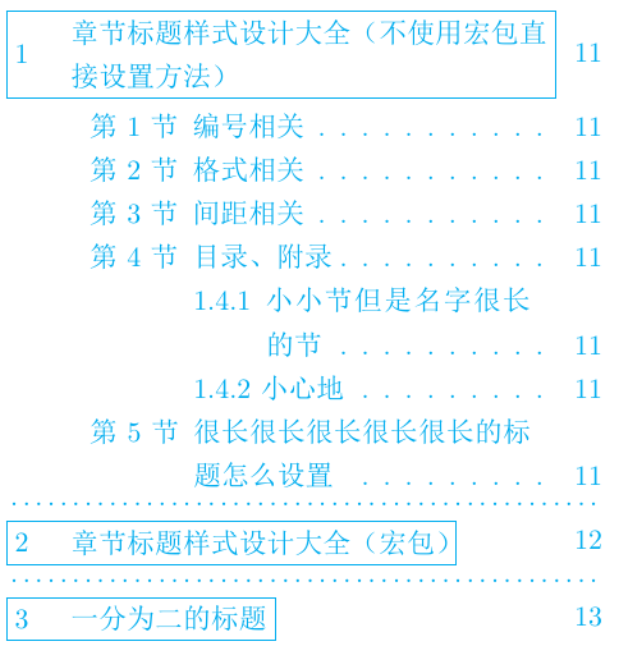
\includegraphics[height=4cm,keepaspectratio]{images/PixPin_2024-10-17_15-56-33.png}}
        \end{minipage}
        }
        % 教育背景
        \begin{minipage}[t]{\textwidth}
        \section[教育背景]{\makebox[\iconwidth][c]{\color{main}{\faGraduationCap}}\quad 教育背景}
        
        % {\large \textbf{宁波大学}},专科 \hfill 2000年9月--2010年6月
        % \begin{itemize}
        %     \item 你的学院,你的专业
        %     \item \textbf{主修课程}:课程1、课程2、课程3、课程4\ 等。
        % \end{itemize}
        
        % \vspace{0.5em}
        {\large \textbf{XX工业大学}},\texttt{本科} \hfill \textbf{2017年9月--2022年7月}
        \begin{itemize}
            \item \textit{理学院,数学与应用数学}
            \item \textbf{主修课程}:数学分析、高等代数、解析几何、常微分方程、概率论、复变函数论、实变函数论、微分几何、科学计算引论、数学物理方程、近世代数、拓扑学、泛函分析等。
            % \item \textbf{GPA}:2.5 / 4.8%(排名:1 / 250)
        \end{itemize}
        \vspace{-.5em}\tikz\draw[line width=0.5pt,dashed,main] (0,0)--++(\textwidth,0);\\
        {\large \textbf{XX大学}},\texttt{硕士} \hfill \textbf{2022年9月--至今}
        \begin{itemize}
            \item \textit{数学与物理学院,现代微分几何}
            \item \textbf{研究方向}:复几何、复分析、微分几何\ 等。
        \end{itemize}
        
        \vspace{1.2em}
        \end{minipage}

    \begin{minipage}[t]{\textwidth}
    % 科研成果
    \section[科研成果]{\makebox[\iconwidth][c]{\color{main}{\faAtom}}\hspace{1em} 科研成果}

    % 科研著作(研究生)
    \begin{itemize}
        \item     Logarithmic vanishing theorems on weakly $1$-complete K\"ahler manifolds, Shilong Lu. \hfill \textbf{在投} 
        \begin{itemize}[]
            \item We give a new type log vanishing theorem on weakly 1-complete K\"ahler manifolds.
        \end{itemize}
    \end{itemize}

    \vspace{0.5em}

    \begin{itemize}
        \item     Extension theorem for jets on weakly pseudoconvex K\"ahler manifolds, Shilong Lu. \hfill \textbf{在投} 
        \begin{itemize}[]
            \item We find a new $L^q$-extension theorem on weakly pseudoconvex K\"ahler manifolds.
        \end{itemize}
    \end{itemize}
    
    \vspace{1.2em}
    \end{minipage}

    % \begin{minipage}[t]{\textwidth}
    % % 项目经历\科研经历\项目与教学(标题请根据需要修改)
    % \section[项目与教学]{\makebox[\iconwidth][c]{\color{main}{\faChalkboardTeacher}}\quad 项目与教学}
    
    % {\large \textbf{项目名称}} \hfill 2020年9月--2021年9月
    % \begin{itemize}
    %     \item \textbf{你在项目中扮演的角色} \hfill 横向/纵向项目-已完结/进行中
    %     \item 用一句话介绍你在这个项目中做了什么\dots\dots
    % \end{itemize}

    % \vspace{0.5em}
    % {\large \textbf{某某主题讨论班}},主讲 / 参与 \hfill 2020年夏季
    % \begin{itemize}
    %     \item \textbf{主要内容}:内容1,内容2,内容3\ 等。
    % \end{itemize}

    % \vspace{0.5em}
    % {\large \textbf{课程名称}},助教 \hfill 2021年夏季
    % \begin{itemize}
    %     \item \textbf{主要内容}:内容1,内容2,内容3\ 等。
    % \end{itemize}
    
    % \vspace{1.2em}
    % \end{minipage}
    
    % 如果每行的内容不是很多,可以考虑使用 minipage,将内容分列展示
    \begin{minipage}[t]{0.6\textwidth}
        \section[技能特长]{\makebox[\iconwidth][c]{\color{main}{\faWrench}}\quad 技能特长}
        \begin{itemize}
        \setlength{\itemsep}{0.5em}
            \item 熟练使用 \LaTeX 进行科学排版。
            \item 熟悉 WPS 和 Office 软件使用。
            \item 掌握 Mathematica 和 Matlab 等软件使用方法。
            \item 英语六级。
        \end{itemize}
    \end{minipage}
    \hfill
    \begin{minipage}[t]{0.35\textwidth}
        \section[兴趣爱好]{\makebox[\iconwidth][c]{\color{main}{\faStar}}\quad 兴趣爱好}
        \begin{itemize}
        \setlength{\itemsep}{0.5em}
            \item \LaTeX 排版
            \item 计算机技术
            \item 打羽毛球和跑步
            \item 文学与诗词
        \end{itemize}
    \end{minipage}

    \vspace{1.2em}
    \begin{minipage}[t]{\textwidth}
        % 项目经历\科研经历\项目与教学(标题请根据需要修改)
        \section[自我评价]{\makebox[\iconwidth][c]{\color{main}{\faChalkboardTeacher}}\quad 自我评价}
具有良好的教师职业操守和服务意识,热爱教育教学工作,热爱学生,沟通表达能力强,讲课条理清晰,风趣幽默,有互动,能够因材施教,启发教学, 善于总结学科学习的重难点,有能力帮助学生提高学分,有责任心,上进心,良好的沟通能力。
    \end{minipage}
    % \newpage
    % % 如有需要,可以添加额外的页面。不要忘记添加页眉页脚和背景相关的代码。

    % % 竞赛经历
    % \section{\makebox[\widthof{\faTrophy}][c]{\color{main}{\faTrophy}}\quad 竞赛经历}
    % \begin{table}[h!]
    %     \begin{tabularx}{\textwidth}{Xp{\widthof{第零负责人}}p{\widthof{国家级-第100名}}p{\widthof{2030年13月}}}
    %         \textbf{比赛1} & 第一负责人 & 国家级-第10名 & 2023年4月 \\
    %         \textbf{比赛2} & 个人参赛 & 国家级-一等奖 & 2023年8月\\
    %         \textbf{比赛3} & 个人参赛 & 省级-一等奖 & 2022年12月\\
    %         % 同理,可以自己加
    %     \end{tabularx}
    % \end{table}

    % % 技能特长
    % \section{\makebox[\widthof{\faWrench}][c]{\color{main}{\faWrench}}\quad 技能特长}
    % \begin{itemize}
    %     \item 熟练使用\Cpp 、Python、Matlab编程语言。
    %     \item 熟悉Windows与Linux端开发。
    %     \item 熟练使用Tensorflow,Pytorch等深度学习框架。
    %     \item 熟练掌握\Cpp 与Python环境下OpenCV与Qt应用的开发,且熟练使用Qt Creator软件。
    %     \item 熟练使用Altium Designer与LCEDA进行封装绘制与板子设计。
    %     \item 熟练使用Keil,Arduino IDE等集成开发软件。
    %     \item 了解模式识别,强化学习,遗传算法,知识蒸馏等相关概念。
    % \end{itemize}

    % % 所获荣誉
    % \section{\makebox[\widthof{\faStar}][c]{\color{main}{\faStar}}\quad 所获荣誉}
    % \begin{multicols}{2}
    %     \begin{itemize}
    %         \item 某年学业先进个人
    %         \item 某年某奖学金某等奖
    %         \item 某大使
    %         \item 某年某奖学金某等奖
    %         \item 某年优秀团员称号
    %         \item 某年某称号
    %     \end{itemize}
    % \end{multicols}

    % % 其他
    % \section{\makebox[\widthof{\faInfo}][c]{\color{main}{\faInfo}}\quad 其他}
    % \begin{itemize}
    %     \item 英语水平-CET6级xxx分
    %     \item 计算机几级证书
    %     \item xx几级证书
    %     \item 技术博客: 某网址
    %     \item 教师资格证:xxx
    %     \item 普通话证书:几级几等
    %     \item 文字排版:\LaTeX
    % \end{itemize}

\end{document}
